% ------------------------------------------------------------------------------
% TYPO3 Version 11.1 - What's New (German Version)
%
% @license	Creative Commons BY-NC-SA 3.0
% @link		http://typo3.org/download/release-notes/whats-new/
% @language	German
% ------------------------------------------------------------------------------
% Feature | 93526 | Multi-Factor Authentication (1)

\begin{frame}[fragile]
	\frametitle{Änderungen für Integratoren und Entwickler}
	\framesubtitle{Multi-Faktor-Authentifizierung (1)}

	\lstset{basicstyle=\fontsize{8}{10}\ttfamily}

	\begin{itemize}
		\item TYPO3 v11.1 bietet
			\href{https://en.wikipedia.org/wiki/Multi-factor_authentication}{Multi-Faktor-Authentifizierung}.
		\item Der TYPO3 Core enthält standardmäßig zwei MFA-Anbieter::

			\begin{itemize}
				\item Zeitbasiertes Einmal-Passwort (TOTP)
				\item Wiederherstellungscode (\textit{fallback provider})
			\end{itemize}

	\end{itemize}

	\begin{figure}
		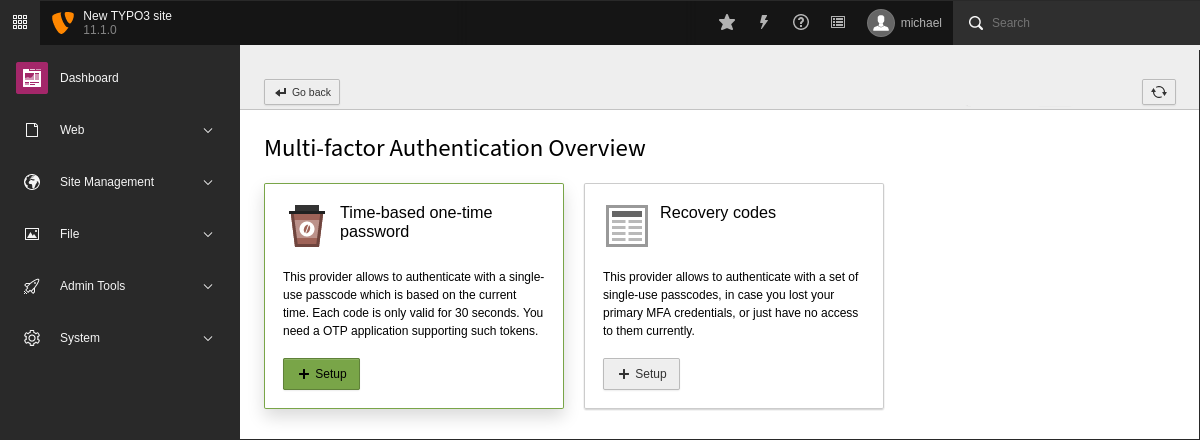
\includegraphics[width=0.8\linewidth]{ChangesForIntegratorsAndDevelopers/1613731375-MultiFactorAuthentication.png}
	\end{figure}

\end{frame}

% ------------------------------------------------------------------------------
